% --------------------------
% Vortrag:
% Überblick über die Absicherung von DNNs im autonomen Fahren
% 2018-12-20
%
% Gesina Schwalbe,
% Kolloquium des Lehrstuhls KogSys, Fakultät WIAI, Universität Bamberg
%
% - Inhalt -
% ---------------------------

\usepackage{fontspec}
\usepackage{lmodern}
\usepackage[shorthands=off]{babel}
\usepackage{csquotes}
\usepackage{graphicx}
\graphicspath{{./images/}}
% \usepackage{mathtools}
\usepackage{booktabs}

\usepackage[backend=biber,
style=numeric,
doi=false
]{biblatex}
\renewcommand*{\bibfont}{\tiny}
\bibliography{DNN-Absicherung.bib}


\title{DNN-Absicherung}
\subtitle{Ein Überblick}
\author{Gesina Schwalbe}
\date{20.~Dezember~2018}

\begin{document}

% title and table of contents
\frame{\maketitle}
\frame{\tableofcontents[hideallsubsections]}

% ------
\enlargethispage{2eM}
\begin{abstract}
Viele herkömmlichen Methoden zur Sicherstellung der Betriebssicherheit
sind auf autonome Fahrzeuge mit DNNs nicht (direkt) anwendbar.
Der Vortrag zu diesen Notizen ist ein Schnelldurchlauf durch die
wichtigsten Fragestellungen und Unterschiede, den aktuellen Stand und
mögliche Ausblicke zur Absicherung von DNNs.
Das Ergebnis ist, dass in allen Phasen, d.h. für Entwicklungsstandards,
Korrekturmethoden, Absicherung während des Betriebs, sowie
problemspezifische Analyse- und Nachweismethoden, Handlungsbedarf
herrscht. Dabei stellen die Analyse und die Betriebsabsicherung
bisher quasi ungelöste Nadelöhre dar.
\end{abstract}


\section{Herkömmlicher Sicherheitsnachweis}
% Orientiert an ISO\,26262 Norm

\subsection{Bestandteile}
\begin{frame}\frametitle<presentation>{\insertsubsection}
  Ein Sicherheitsnachweis eines Kotrollsystems kann/sollte enthalten:
  \begin{description}[]
  \item[Gefahren- und Risikoanalyse]
    \mode<article>{zur Bestimmung von Sicherheitsanforderungen
      \begin{itemize}
      \item Was für Gefahren können auftreten?
      \item Wie wahrscheinlich und wie schwerwiegend sind diese?
      \item Welche kombinierten (Fehl-)Funktionen können dazu führen?
      \item Wer/welcher Systemteil ist für die Verhinderung/Milderung zuständig?
      \end{itemize}
    }
  \item[Nachweise] der identifizierten Sicherheitsanforderungen
    \mode<article>{bzw. Einstufung, wie sicher es ist durch z.B.
      \begin{itemize}
      \item Formale Methoden
      \item Tests
      \end{itemize}
    }
  \item[Präventions-/Milderungsmaßnahmen] für Entwicklung \& Betrieb
  \end{description}
\end{frame}

\mode<article>{
  \subsection{Nachteile}
  Die konventionellen Methoden haben u.a. folgende Nachteile für die
  Anwendung auf AI-Systeme:
  \begin{itemize}[<.->]
  \item Die Risikolevel sind \emph{hardwareorientiert},
    z.B. wird eine gleichverteilte Ausfallwahrscheinlichkeit angenommen
  \item Es wird ein \emph{White-Box}-System benötigt, um mögliche
    Ausfälle bis auf überprüfbare Einzelkomponenten und deren
    (prüfbares) Zusammenspiel zurückverfolgen zu können.
  \end{itemize}
}

\subsection{Typische Methoden}
\begin{frame}\frametitle<presentation>{\insertsubsection}
  \begin{itemize}
  \item Gefahren-/Risikoanalyse
    \mode<article>{(Sind gefährliche Ein-Ausgabe-Kobinationen möglich?)}
    \begin{description}[<.->][]
    \item[Deduktiv] (Rückverfolgung, d.h. starte mit Ausgabewert)
      \mode<article>{\cite{johnson_increasing_2017}}
    \item[Induktiv] (Eingaberaumsuche, d.h. starte mit Eingabewerten)
      \mode<article>{\cite{johnson_increasing_2017}}
    \item[Vollständiges Testen]
    \item[Bewährtheit im Betrieb]
    \end{description}
  \item Prävention/Milderung
    \begin{description}[<.->][]
    \item[Überwachung]
    \item[Backupsysteme]
    \item[Saubere Entwicklung]
    \item[Safety-Life-Cycle]
    \end{description}
  \end{itemize}
\end{frame}

\mode<article>{
  \subsection{Unterschiede von ML-Systemen}
  \begin{description}[]
  \item[Komplexität des Problems und Black-Box Natur]~
    \begin{itemize}
    \item Wenig Verständis von Randbereichen des Algorithmus
      \begin{itemize}
      \item Wann befinden sich die Ein- oder Ausgaben außerhalb des
        (sicheren) Betriebsbereichs? Wie sieht effektive Überwachung aus?
      \item Keine Bewährung durch langen Betriebseinsatz
      \end{itemize}
    \item Große Ein- und Zustandsbereiche, dazu wenig Wissen über den
      Entscheidungsprozess (den Kontrollfluss)
      \begin{itemize}
      \item Keine deduktiven Methoden
      \item Keine induktiven Methoden
      \item Kein vollständiges Testen
      \end{itemize}
    \item Komplexität des Algorithmus
      \begin{itemize}
      \item Wie erkennt man da noch Implementierungsfehler?
      \end{itemize}
    \end{itemize}

  \item[Keine Qualitätskriterien], die allg. anerkannt sind, u.a.
    \begin{itemize}
    \item Metriken und entsprechende Schwellenwerte
    \item Systematische Maßnahmen zur Erkennung gängier Fehler
    \item Stand der Technik (d.h. Faustregeln) für Entwicklung und
      Betrieb; vollständiger Lebenszyklus (d.h. Plan für
      Zwischenschritte mit Qualitätsmanagement)
    \end{itemize}

  \item[Neue Komponenten] kommen zum Einsatz, z.B.
    \begin{itemize}
    \item Bibliotheken
    \item Spezialisierte Hardware, z.B. Neuromorphic Chips
    \end{itemize}
  \end{description}
}

\section[Offene Fragen]{Offene Fragen für das Fehlermanagement}
Für einen vollständigen Sicherheitsnachweis müssen in jeder Phase des
Lebenszyklus bestmögliche Maßnahmen ergriffen werden, um (gefährliche)
Fehler zu vermeiden.

\mode<article>{\subsection{Scope des Vortrags}}
Beim automatisierten Fahren wird in
Wahrnehmungsaufgaben (Computer Vision) und Planungs-
bzw. Entscheidungsaufgaben unterschieden
\cite{fernandes_rational_2017}.
Der Bereich der Planungs- und Entscheidungsaufgaben
ist bereits gut durch Überwachung abgedeckt:
\begin{itemize}
\item Einfaches Beispiel: \cite{fernandes_rational_2017}
\item Vollständiges Verhaltensregelwerk:
  \cite{shalev-shwartz_formal_2017}
\item Existenzbeweis: \cite{lygeros_controllers_1999}
\item Regelerlernen und Überwachung für Reinforcement Learning:
  \cite{ghosh_trusted_2016,akametalu_reachability-based_2014,fridovich-keil_planning_2017}
\end{itemize}
Daher konzentriert sich die folgende Analyse auf Wahrnehmungsaufgaben.

\begin{frame}\frametitle<presentation>{\insertsubsection}
  \begin{figure}
    \centering
    \parbox{.4\linewidth}{
      \href{https://raw.githubusercontent.com/matterport/Mask_RCNN/master/assets/street.png}%
      {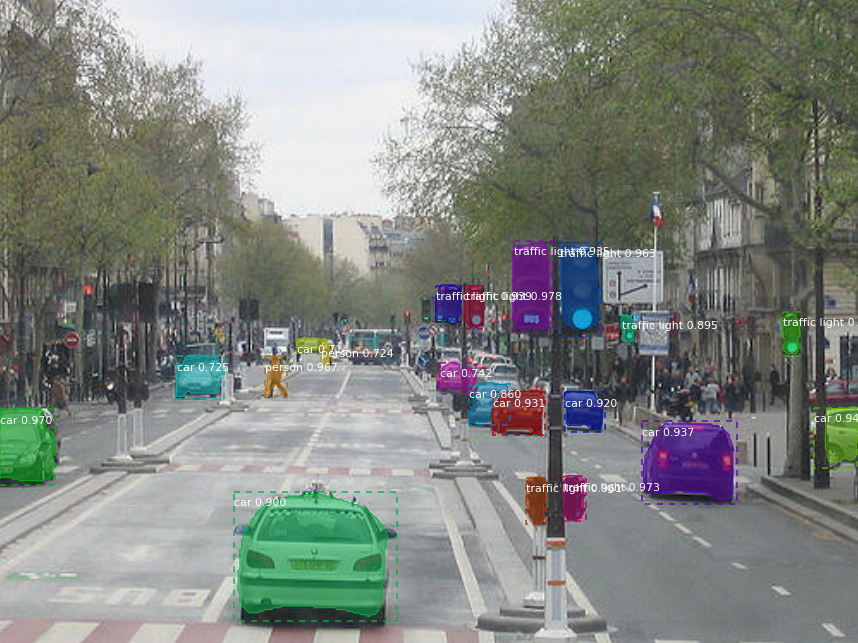
\includegraphics[width=\linewidth]{computer_vision}}
      \mode<article>{\caption{Typischer Teil der Wahrnehmungsaufgaben:
        Segmentierung der Kameraaufnahmen}}
    }\hspace{0.1\linewidth}
    \parbox{.4\linewidth}{
      \href{https://sites.google.com/view/waymo-learn-to-drive/}%
      {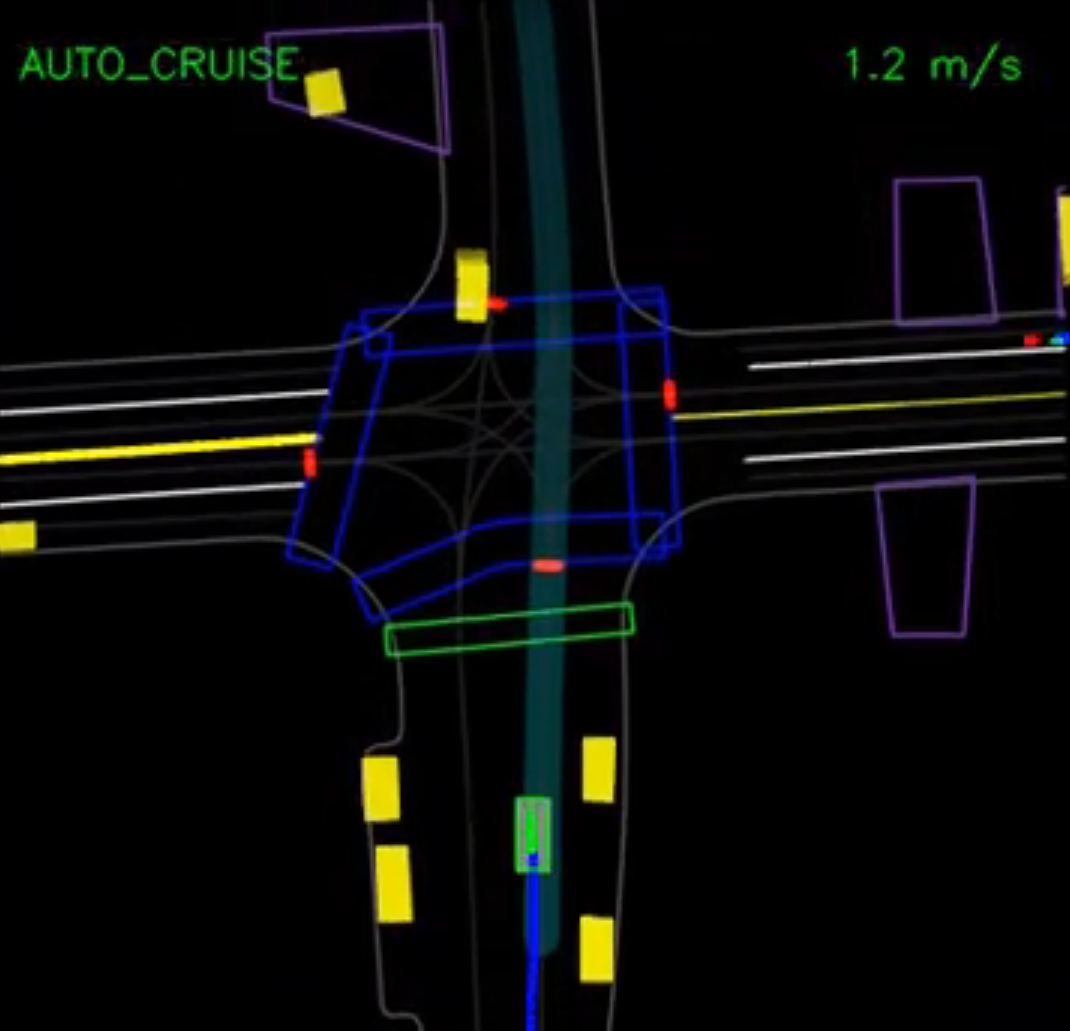
\includegraphics[width=\linewidth]{planning}}
      \mode<article>{\caption{Typischer Input für
          Planungs-/Entscheidungsaufgaben wie z.B. Trajektorienplanung}}
    }%
  \end{figure}
\end{frame}

Die übergeordneten Phasen sind
Entwicklung,
Prüfung,
Korrektur,
Betrieb.
Entwicklung, Prüfung und Korrektur bilden einen Zyklus.
Die Prüfung kann unterteilt werden in
\begin{itemize}
\item Risikoprüfung bzw. Formulierung von Sicherheitskriterien und
\item Prüfen dieser.
\end{itemize}
\begin{frame}\frametitle<presentation>{Phasen im Fehlermanagement}
  \begin{figure}
    \centering
    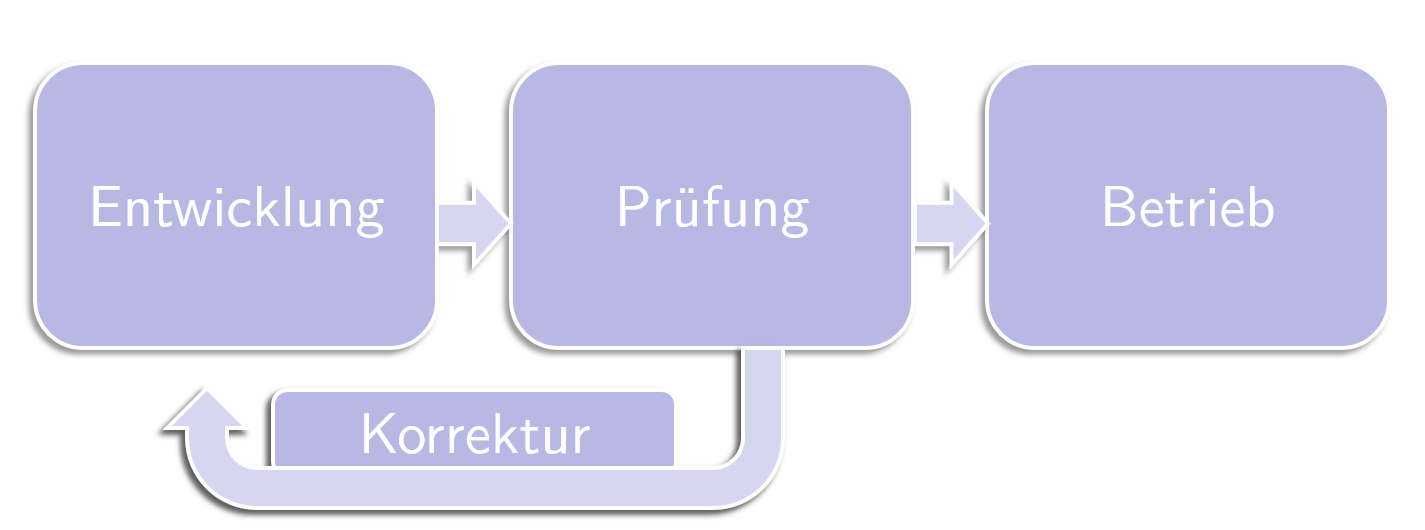
\includegraphics[width=\textwidth]{lifecycle}
    \mode<article>{\caption{
        Phasen des Lebenszyklus eines Systems, die relevant für das
        Fehlermanagement sind.
      }}
  \end{figure}
\end{frame}


\subsection{Wie erkennt/verhindert man Fehler frühzeitig?}
\mode<presentation>{
  \begin{frame}\frametitle{\insertsubsection}
    \begin{figure}
      \centering
      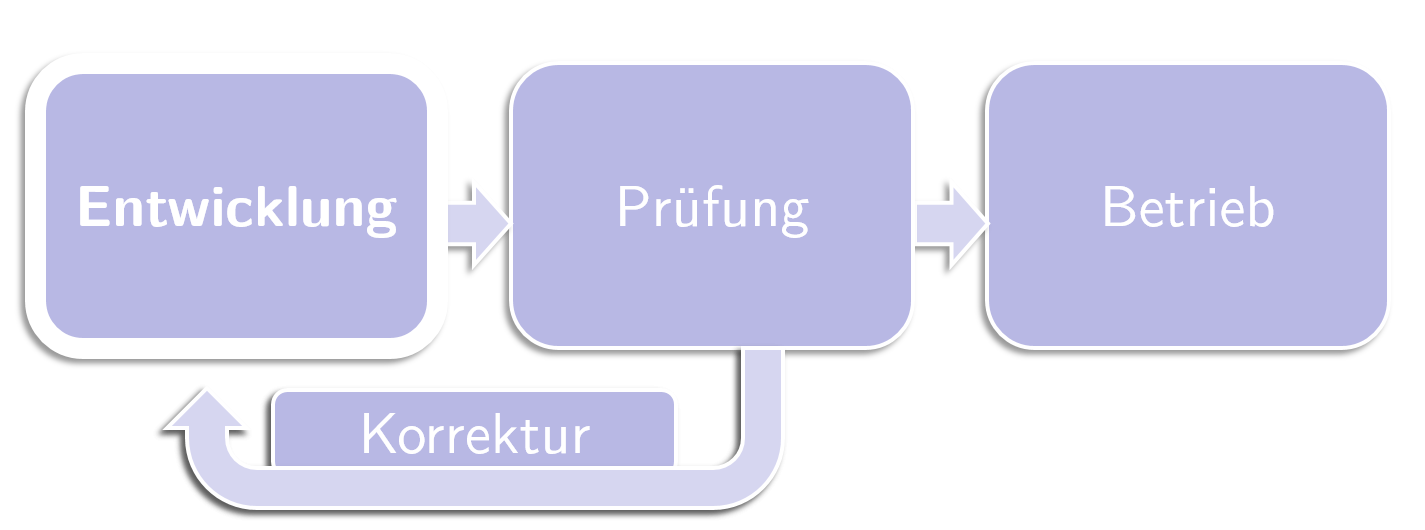
\includegraphics[width=\linewidth]{lifecycle1}
    \end{figure}
  \end{frame}
}
Die aktuellen ISO Normen zum Thema Absicherung geben nicht nur
Empfehlungen zum Überprüfungsprozess, sondern generell eine
Sammlung (damaliger) Prozessstandards wider. Das schließt für Software
z.B. Unittests mit Abdeckungsmetriken, sinnvolle Modularisierung und
Variablenbenennung mit ein.
Für neuartige Entwicklungsbestandteile von AI fehlen allerdings solche
Faustregeln.

\begin{frame}\frametitle<presentation>{Ansätze für Faustregeln und Metriken}
  \begin{description}[Design] % für 16:9 [Lern-Daten \emph{(Datenrepräsentativität)}] sonst [Desing]
  \item[Lern-Daten \emph{(Datenrepräsentativität)}]
    Betonung von Gegenbeispielen und relevanten Szenarien
  \item[Test-Daten \emph{(Testabdeckung)}]
    sicherheitsrelevante Testabdeckung,
    z.B. Concolic Testing~\cite{youcheng_concolic_2018}
  \item[Robustheit \emph{(Robustheitsgrad)}]
    Dropout, Regularisierung, Robust Manifold Ansatz, Adversarial Learning, \dots
  \item[Plausibilisierung]
    Funktionalitätsprüfung für designspezifische Probleme, z.B. Reward-Hacking
  \item[Expertenwissen \emph{(Regelbefolgung)}] einfügen
  \item[Design]
    Faustregeln zu Loss-/Reward-Funktion, Layern, Aktivierungen,
    Ungewissheitsangaben \dots
  \end{description}
\end{frame}
Es gilt also, die bisherigen Entwicklungsstandards, wenn nötig,
auszubauen, brauchbare Metriken zu formulieren und einem Standard hinzuzufügen.


\subsection{Wie findet man gefährliche Fehler(ursachen)?}
\mode<presentation>{
  \begin{frame}\frametitle{\insertsubsection}
    \begin{figure}
      \centering
      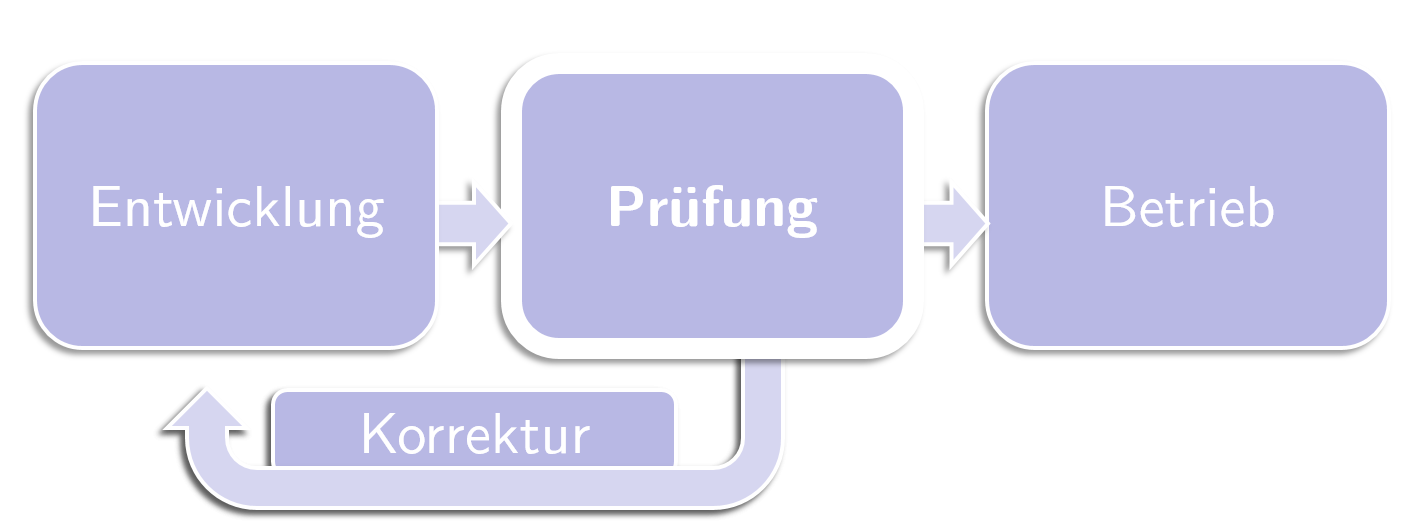
\includegraphics[width=\linewidth]{lifecycle2}
    \end{figure}
  \end{frame}
}
\begin{frame}\frametitle<presentation>{\insertsubsection}
  Zur Analyse auf problemspezifische Fehler hin ist ein
  \emph{White-Box}-System nötig! Hoffnung:
  \begin{description}[<.->]
  \item[Eingrenzung] der Ein-/Zustandsbereiche
  \item[Vereinfachung] des Problems durch Abstrahierung
  \end{description}
\end{frame}
Leider gibt es bisher keinen vollständigen anwendbaren Ansatz,
mithilfe dessen genügend aussagekräftige, konkrete, durch Regelprüfer
nachweisbare Sicherheitsanforderungen formuliert werden könnten.
Das Problem hierbei ist einerseits die Einsicht in den Algorithmus,
andererseits die Übersetzung von qualitativen/in natürlicher Sprache
formulierten Anforderungen in Bedingungen auf
Eingabe-/Ausgabe-/Zwischenwerten.

\begin{frame}[t]\frametitle{Qualitative Einsicht}
  \begin{description}[<only@+->][]
  \item[Heatmapping] z.B.
    \begin{itemize}[<.->]
    \item LIME~\cite{ribeiro_why_2016},
      RISE~\cite{petsiuk_rise:_2018},
      Instancewise Feature Selection~\cite{chen_learning_2018},
      \dots
    \item LRP~\cite{bach_pixel-wise_2015},
      Attention Visualization~\cite{kim_interpretable_2017},
      \dots
    \end{itemize}
    \only<.>{
      \begin{figure}
        \centering
        \href{https://indico.scc.kit.edu/event/344/contributions/2434/attachments/1258/1759/Talk_Samek.pdf}%
        {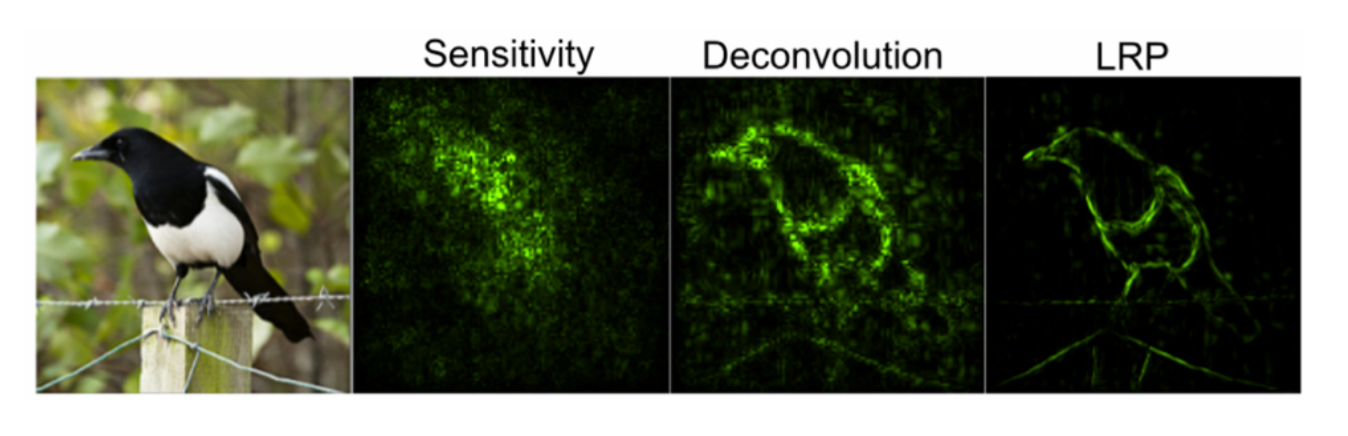
\includegraphics[width=0.6\linewidth]{heatmapping}}
        \mode<article>{\caption{Vergleich verschiedener Heatmapping-Methoden}}
      \end{figure}
    }
  \item[Unsicherheitsangaben] z.B. durch
    \begin{itemize}[<.->]
    \item spezielle Backpropagation~\cite{gast_lightweight_2018}
    \item erlernten Weight Decay~\cite{kendall_what_2017}
      \only<.>{
      \begin{figure}
        \centering
        \href{http://arxiv.org/abs/1703.04977}%
        {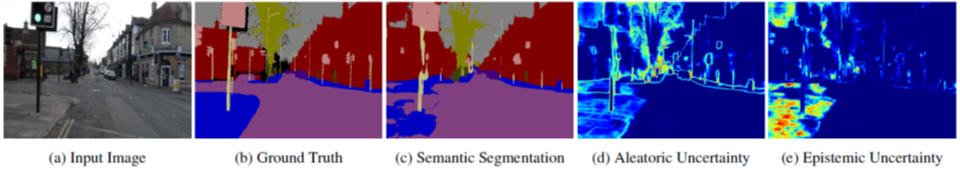
\includegraphics[width=\linewidth]{learned_weight_decay}}% für 16:9 0.9\linewidth, sonst 1
        \mode<article>{\caption{Ausgabe und Visualisierung von
            Unsicherheit mit erlerntem Weight
            Decay~\cite{kendall_what_2017}. Die falsche Segmentierung
            des Gehwegs (c) sowie Kanten von Segmentierungsobjekten
            werden als stark ungewisse Zonen in der Ausgabe markiert (e).}}
      \end{figure}
    }
  \end{itemize}
  \item[Aufgabenlokalisierung] z.B. durch
    Neural Stethoscopes~\cite{fuchs_neural_2018}
    \only<.>{
      \\<presentation>
      \begin{figure}
        \centering
        \href{https://arxiv.org/abs/1806.05502v2}%
        {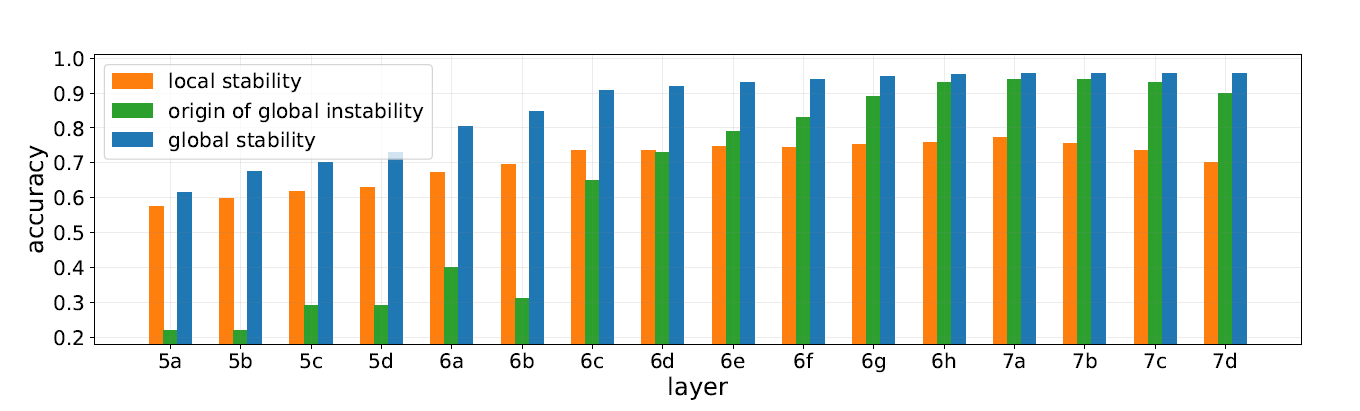
\includegraphics[width=0.6\linewidth]{neural_stethoscopes}} % für 16:9 0.4\linewidth, sonst 0.6
        \mode<article>{\caption{Anwendung von Neural Stethoscopes, um
            bei einem Stabilitätsvorhersageproblem die
            Layerzuständigkeit für einzelne Unteraufgaben zu
            bestimmen. Je höher die Accuracy für ein Layer, desto besser
            ist der Abstraktionsgrad dieses Layers für diese
            Unteraufgabe geeignet.}}
      \end{figure}
    }
  \item[Netzwerkvereinfachung] z.B. CAR-Compression~\cite{abbasi-asl_interpreting_2017}
    \mode<article>{(ist zumindest hilfreich)}
  \end{description}
\end{frame}

\begin{frame}\frametitle{Regelextraktion}
  \begin{description}[]
  \item[Hauptkriterien] \emph{Verständlichkeit} bei
    \emph{Originaltreue}
  \item[Extrahierte Regeln] Meist \emph{IF-THEN} oder \emph{M-von-N}
  \item[Kategorien:]~
    \begin{description}[<.->][White-/Grey-Box]
    \item[Black-Box] \mode<article>{oder pädagogisch:}
      Verhaltensnachbildung durch Regeln,
      \\<presentation>
      z.B. lokal mit ILP~\cite{rabold_explaining_2018}
    \item[White-/Grey-Box] \mode<article>{oder decompositional/eklektisch:}
      Umwandlung in Entscheidungsbaum,
      \\<presentation>
      z.B. DeepRED~\cite{ruben_zilke_deepred_2016}
    \end{description}
    \mode<article>{Beide Richtungen haben Vor- und
      Nachteile. Pädagogische Methoden erzeugen häufig genauere
      Modelle der ursprüngliche Funktion, sind dafür aber meist weniger
      effizient \cite{davila_garcez_symbolic_2001}.
    }
  \end{description}
\end{frame}

\subsection{Wie weist man Fehlerfreiheit nach?}
\mode<presentation>{
  \begin{frame}\frametitle{\insertsubsection}
    \begin{figure}
      \centering
      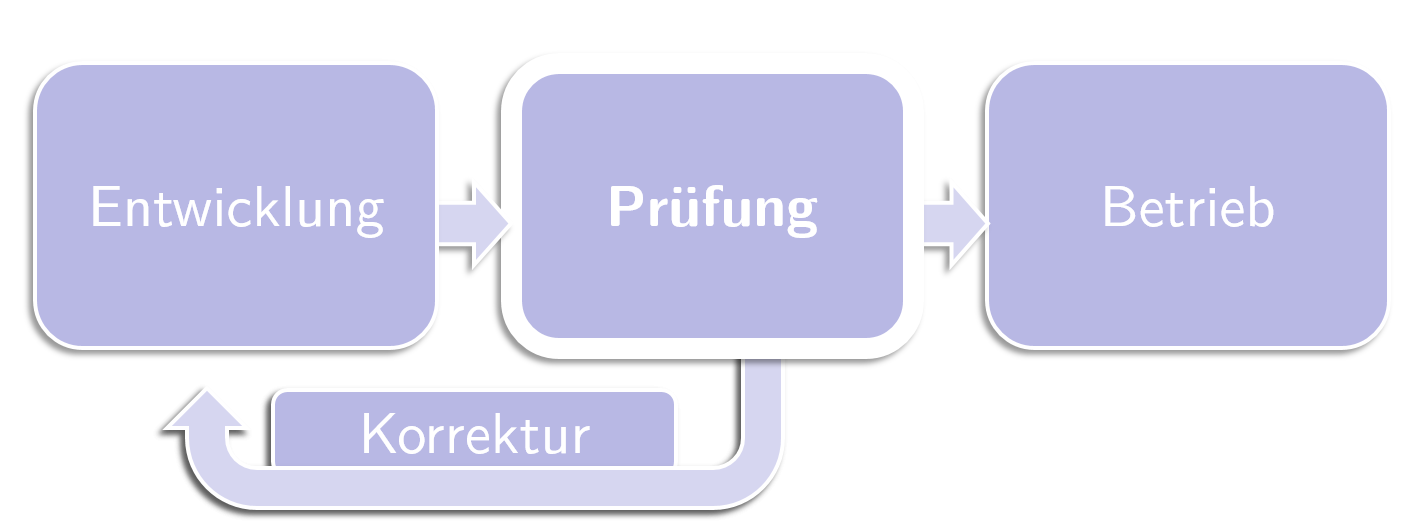
\includegraphics[width=\linewidth]{lifecycle2}
    \end{figure}
  \end{frame}
}

Die Alternativen sind:
\begin{frame}\frametitle<presentation>{\insertsubsection}
  \begin{itemize}
  \item Manuell
  \item Automatisch
    \begin{description}[]
    \item[Entscheidungsproblemlöser] z.B.
      Reluplex~\cite{katz_reluplex:_2017} (SMT),
      \cite{huang_safety_2016} (SMT), % satisfiability modulo theory
      SHERLOCK~\cite{dutta_output_2017} (MILP) % mixed integer linear programming
    \item[Randannäherung] z.B.
      DeepGo~\cite{ruan_reachability_2018},
      ReluVal~\cite{wang_formal_2018},
      NeVer~\cite{pulina_abstraction-refinement_2010}
    \item[Suchalgorithmen] z.B.
      VeriVis~\cite{pei_towards_2017}      
    \end{description}
  \end{itemize}
\end{frame}
Damit existieren machbare Ansätze für Regelprüfung, welche allerdings
entweder schlecht skalieren (z.B. Reluplex) oder bezüglich der
prüfbaren Regeln sehr eingeschränkt sind (z.B. nur Adversarial Examples).

\subsection{Wie korrigiert man Fehler?}
\mode<presentation>{
  \begin{frame}\frametitle{\insertsubsection}
    \begin{figure}
      \centering
      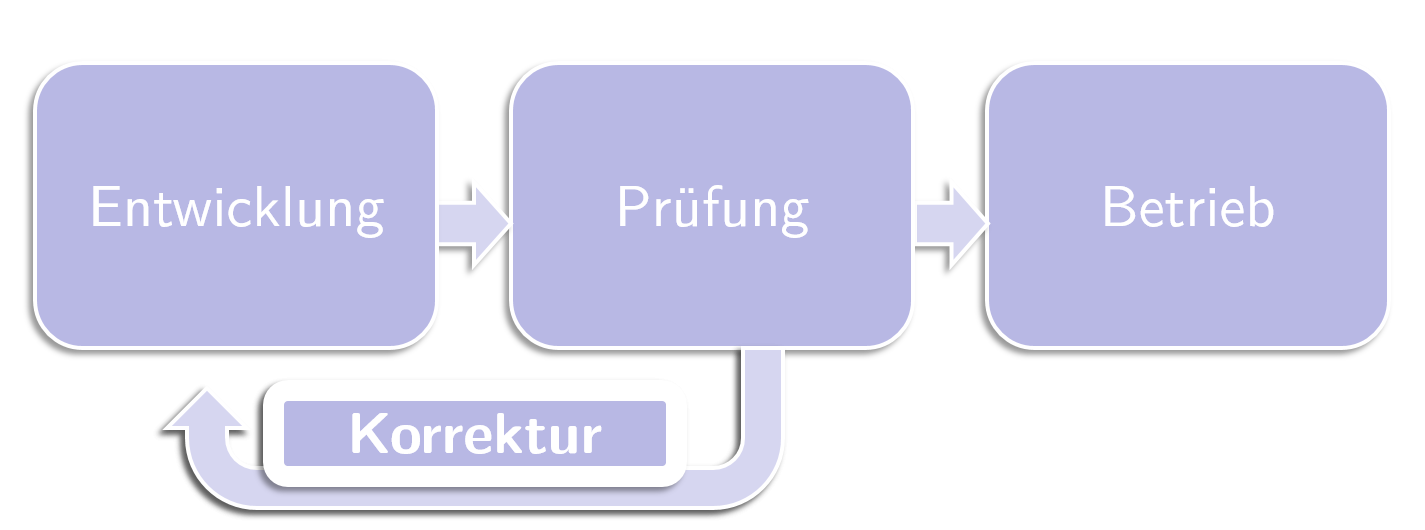
\includegraphics[width=\linewidth]{lifecycle3}
    \end{figure}
  \end{frame}
}

\begin{frame}\frametitle<presentation>{\insertsubsection}
  \begin{description}[Neue Daten]
  \item[Anlernen] Modifiziere Loss- oder Reward-Funktion,
    \\<presentation> z.B.
    \cite{roychowdhury_image_2018},
    Teacher Network~\cite{hu_harnessing_2016},
    Model Repair~\cite{ghosh_trusted_2016}
  \item[Anpassen der Topologie] z.B.
    KBANN~\cite{opitz_heuristically_1993} oder ReNN~\cite{wang_renn:_2018}
    \mode<article>{\\Bei KBANN wird ein kleines Netze aus einem
      Entscheidungsbaum konstruiert, während bei ReNN ein Netz zerlegt
      wird in Abstraktion, Regeln auf abstrakten Features,
      Entscheidung.}
  \item[Neue Daten] Lernen mit Gegenbeispielen,
    \\<presentation>
    z.B. erstellt von Regelprüfern oder mit
    \cite{%
      dreossi_counterexample-guided_2018,% framework
      youcheng_concolic_2018,% concolic testing
      guo_dlfuzz:_2018,% DLFuzz
      he_decision_2018% OptMargin
      })
  \end{description}
\end{frame}
Passend auf Eingabe-/Ausgabe-/Zwischenwerten formulierte
Anforderungen können demnach in die Netzwerkfunktionalität selbst
eingebaut werden. Die verfügbaren Methoden geben jedoch keine Garantie
über den Erfolg des Einfügens, welcher mit einem Regelprüfer evaluiert
werden muss.


\subsection{Wie mildert/umgeht man bestehende funktionale Fehler?}
\mode<presentation>{
  \begin{frame}\frametitle{\insertsubsection}
    \begin{figure}
      \centering
      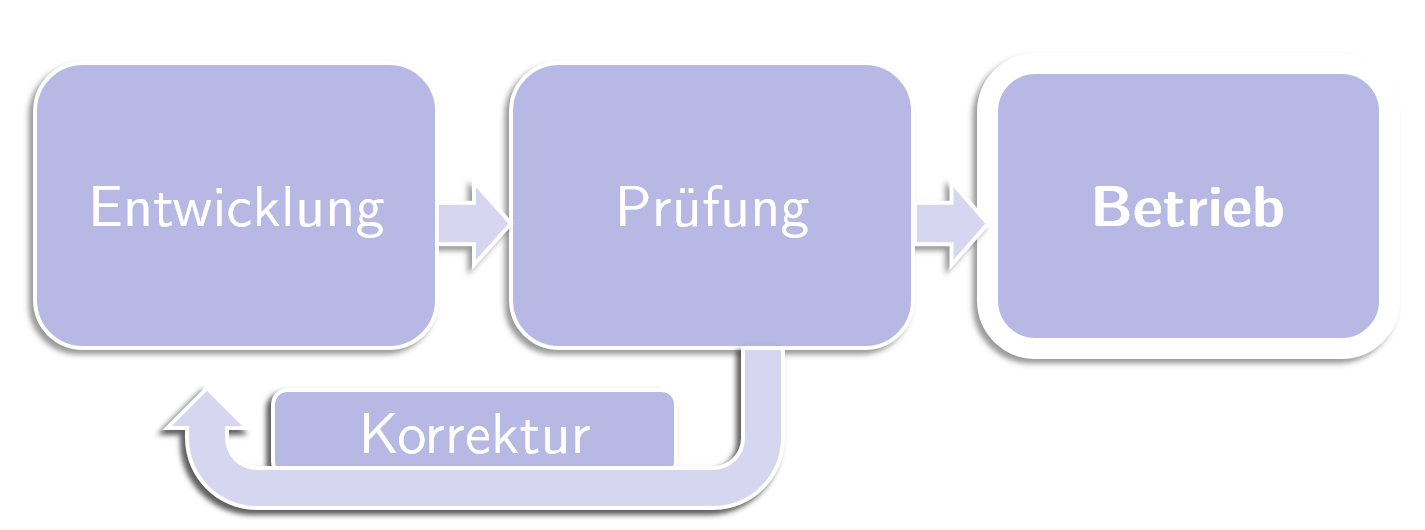
\includegraphics[width=\linewidth]{lifecycle4}
    \end{figure}
  \end{frame}
}

\begin{frame}\frametitle<presentation>{\insertsubsection}
  \begin{description}[]
  \item[Überwachung] d.h. Plausibilisierung für
    \begin{itemize}[<.->]
    \item Eingaben (z.B. Sensorikredundanz \& -abgleich)
    \item Ausgaben (z.B. Bereichs-, Ungewissheitsüberwachung)
    \end{itemize}
  \item[Redundanz]
  \item[Backup-/Fallback-System(e)]
    \emph{fail operational} vs. bisher \emph{fail safe}
    \mode<article>{\\
      Beim automatisierten Fahren muss das Auto
      betriebsfähig bleiben, selbst wenn kleinere Fehler auftreten
      (also keine Vollbremsung auf der Autobahn wegen eines
      Dreckflecks)!
      Bisher ist dieser Teil ungelöst.
    }
  \end{description}
\end{frame}

\subsection{Fazit}
Handlungsbedarf besteht noch in jeder Phase.
Nach aktuellem Stand absteigend sortiert:
\begin{description}
\item[Entwicklung] Hier gibt es einige gute qualitative Ansätze, die
  bereits weithin verbreitet sind. Es fehlt \enquote{nur} die
  Standardisierung sowie eine Quantisierung durch Metriken.
\item[Korrektur] Hier gibt es eine große Lücke bei Ansätzen, die eine
  Garantie über den Erfolg des Regeleinfügens geben. Das kann
  allerdings durch die vielfältigen qualitativen Ansätze in
  Kombination mit passenden Regelprüfern ausgeglichen werden.
\item[Betrieb] Es gibt Ideen zur Überwachung und zur Redundanz,
  allerdings weniger für Computer Vision.
  Die Frage nach einem Fallback-System ist ungeklärt.
\item[Prüfung] Das Nadelöhr hier ist die Risikoanalyse und
  Formulierung prüfbarer Sicherheitskriterien.
  Hier sind hauptsächlich qualitative Ansätze verfügbar,
  und alle weiteren sind bisher nicht für die Verwendung in der
  Sicherheitsprüfung evaluiert.
  Für das Überprüfen von Sicherheitskriterien sind reichlich, wenn
  auch vermutlich noch nicht genügend performante, Methoden
  verfügbar.
\end{description}

\mode<presentation>{
  \begin{frame}\frametitle{\insertsubsection}
    \begin{figure}
      \centering
      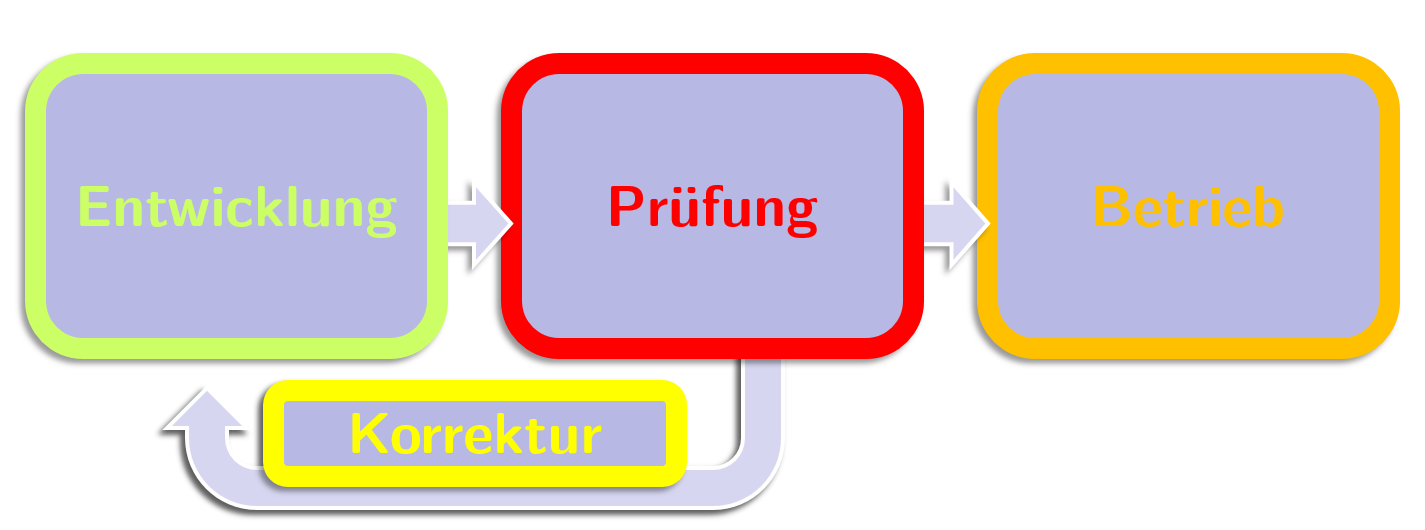
\includegraphics[width=\linewidth]{lifecycle_evaluation}
    \end{figure}
  \end{frame}
}

\mode<presentation>{
\begin{frame}
  \centering
  \Large
  Fragen, Anregungen \dots
\end{frame}
}

\begin{frame}[t,allowframebreaks]
  \frametitle<presentation>{Literaturverzeichnis}
  \tiny
  \printbibliography
\end{frame}



\end{document}



%%% Local Variables:
%%% mode: latex
%%% TeX-master: "DNN-Absicherung_Folien"
%%% ispell-local-dictionary: "en_US"
%%% End:
